%%%%%%%%%%%%%%%%%%%%%%%%%%%%%%%%%%%%%%%%%
% Article EcoFoG
% Version 2.1 (23/10/2017)
%
% adapté de :
% Stylish Article
% LaTeX Template
% Version 1.0 (31/1/13)
%
% This template has been downloaded from:
% http://www.LaTeXTemplates.com
%
% Original author:
% Mathias Legrand (legrand.mathias@gmail.com)
%
% License:
% CC BY-NC-SA 3.0 (http://creativecommons.org/licenses/by-nc-sa/3.0/)
%
%%%%%%%%%%%%%%%%%%%%%%%%%%%%%%%%%%%%%%%%%


%----------------------------------------------------------------------------------------
%	PACKAGES AND OTHER DOCUMENT CONFIGURATIONS
%----------------------------------------------------------------------------------------

\documentclass[fleqn,10pt]{ArtEcoFoG} % Document font size and equations flushed left

\setcounter{tocdepth}{3} % Show only three levels in the table of contents section: sections, subsections and subsubsections


% Pandoc environments
\usepackage{framed}
\usepackage{fancyvrb}
\providecommand{\tightlist}{%
  \setlength{\itemsep}{0pt}\setlength{\parskip}{0pt}}
\newcommand{\VerbBar}{|}
\newcommand{\VERB}{\Verb[commandchars=\\\{\}]}
\DefineVerbatimEnvironment{Highlighting}{Verbatim}{commandchars=\\\{\}, fontsize=\scriptsize} % Code R
\definecolor{shadecolor}{RGB}{248,248,248}
\newenvironment{Shaded}{\begin{snugshade}}{\end{snugshade}}
\newcommand{\KeywordTok}[1]{\textcolor[rgb]{0.13,0.29,0.53}{\textbf{{#1}}}}
\newcommand{\DataTypeTok}[1]{\textcolor[rgb]{0.13,0.29,0.53}{{#1}}}
\newcommand{\DecValTok}[1]{\textcolor[rgb]{0.00,0.00,0.81}{{#1}}}
\newcommand{\BaseNTok}[1]{\textcolor[rgb]{0.00,0.00,0.81}{{#1}}}
\newcommand{\FloatTok}[1]{\textcolor[rgb]{0.00,0.00,0.81}{{#1}}}
\newcommand{\ConstantTok}[1]{\textcolor[rgb]{0.00,0.00,0.00}{{#1}}}
\newcommand{\CharTok}[1]{\textcolor[rgb]{0.31,0.60,0.02}{{#1}}}
\newcommand{\SpecialCharTok}[1]{\textcolor[rgb]{0.00,0.00,0.00}{{#1}}}
\newcommand{\StringTok}[1]{\textcolor[rgb]{0.31,0.60,0.02}{{#1}}}
\newcommand{\VerbatimStringTok}[1]{\textcolor[rgb]{0.31,0.60,0.02}{{#1}}}
\newcommand{\SpecialStringTok}[1]{\textcolor[rgb]{0.31,0.60,0.02}{{#1}}}
\newcommand{\ImportTok}[1]{{#1}}
\newcommand{\CommentTok}[1]{\textcolor[rgb]{0.56,0.35,0.01}{\textit{{#1}}}}
\newcommand{\DocumentationTok}[1]{\textcolor[rgb]{0.56,0.35,0.01}{\textbf{\textit{{#1}}}}}
\newcommand{\AnnotationTok}[1]{\textcolor[rgb]{0.56,0.35,0.01}{\textbf{\textit{{#1}}}}}
\newcommand{\CommentVarTok}[1]{\textcolor[rgb]{0.56,0.35,0.01}{\textbf{\textit{{#1}}}}}
\newcommand{\OtherTok}[1]{\textcolor[rgb]{0.56,0.35,0.01}{{#1}}}
\newcommand{\FunctionTok}[1]{\textcolor[rgb]{0.00,0.00,0.00}{{#1}}}
\newcommand{\VariableTok}[1]{\textcolor[rgb]{0.00,0.00,0.00}{{#1}}}
\newcommand{\ControlFlowTok}[1]{\textcolor[rgb]{0.13,0.29,0.53}{\textbf{{#1}}}}
\newcommand{\OperatorTok}[1]{\textcolor[rgb]{0.81,0.36,0.00}{\textbf{{#1}}}}
\newcommand{\BuiltInTok}[1]{{#1}}
\newcommand{\ExtensionTok}[1]{{#1}}
\newcommand{\PreprocessorTok}[1]{\textcolor[rgb]{0.56,0.35,0.01}{\textit{{#1}}}}
\newcommand{\AttributeTok}[1]{\textcolor[rgb]{0.77,0.63,0.00}{{#1}}}
\newcommand{\RegionMarkerTok}[1]{{#1}}
\newcommand{\InformationTok}[1]{\textcolor[rgb]{0.56,0.35,0.01}{\textbf{\textit{{#1}}}}}
\newcommand{\WarningTok}[1]{\textcolor[rgb]{0.56,0.35,0.01}{\textbf{\textit{{#1}}}}}
\newcommand{\AlertTok}[1]{\textcolor[rgb]{0.94,0.16,0.16}{{#1}}}
\newcommand{\ErrorTok}[1]{\textcolor[rgb]{0.64,0.00,0.00}{\textbf{{#1}}}}
\newcommand{\NormalTok}[1]{{#1}}
\usepackage{longtable,booktabs}
\usepackage{caption}
% These lines are needed to make table captions work with longtable:
\makeatletter
\def\fnum@table{\tablename~\thetable}
\makeatother
% longtable 2 columns
% https://tex.stackexchange.com/questions/161431/how-to-solve-longtable-is-not-in-1-column-mode-error
\makeatletter
\let\oldlt\longtable
\let\endoldlt\endlongtable
\def\longtable{\@ifnextchar[\longtable@i \longtable@ii}
\def\longtable@i[#1]{\begin{figure}[t]
\onecolumn
\begin{minipage}{0.5\textwidth}\scriptsize
\oldlt[#1]
}
\def\longtable@ii{\begin{figure}[t]
\onecolumn
\begin{minipage}{0.5\textwidth}\scriptsize
\oldlt
}
\def\endlongtable{\endoldlt
\end{minipage}
\twocolumn
\end{figure}}
\makeatother

\usepackage{graphicx,grffile}
\makeatletter
\def\maxwidth{\ifdim\Gin@nat@width>\linewidth\linewidth\else\Gin@nat@width\fi}
\def\maxheight{\ifdim\Gin@nat@height>\textheight0.8\textheight\else\Gin@nat@height\fi}
\makeatother
% Scale images if necessary, so that they will not overflow the page
% margins by default, and it is still possible to overwrite the defaults
% using explicit options in \includegraphics[width, height, ...]{}
\setkeys{Gin}{width=\maxwidth,height=\maxheight,keepaspectratio}

% User-adder preamble
\usepackage{textcomp} \DeclareUnicodeCharacter{B0}{\textdegree}
\usepackage{tabu}
\renewenvironment{table}{\begin{table*}}{\end{table*}\ignorespacesafterend}
\hyphenation{bio-di-ver-si-ty sap-lings post-dis-tur-bance}
\hypersetup{draft}

%----------------------------------------------------------------------------------------
%	ARTICLE INFORMATION
%----------------------------------------------------------------------------------------

\JournalInfo{\ }
\Archive{\ }

\PaperTitle{30 Years of Post-disturbance Recruitment in a Neotropical Forest} % Article title

\Authors{
Ariane MIRABEL\textsuperscript{1*}\\ Eric MARCON\textsuperscript{1}\\ Bruno HERAULT\textsuperscript{2}
} % Authors
\affiliation{
\textsuperscript{1}UMR EcoFoG, AgroParistech, CNRS, Cirad, INRA, Université des Antilles,
Université de Guyane.\\ \hspace{1em} Campus Agronomique, 97310 Kourou, France.\\\textsuperscript{2}INPHB (Institut National Polytechnique Félix Houphoüet Boigny)\\ \hspace{1em} Yamoussoukro, Ivory Coast
}
\affiliation{*\textbf{Corresponding author}: ariane.mirabel@ecofog.gf, https://github.com/ArianeMirabel} % Corresponding author

\Keywords{Disturbance Dynamics, Neotropical Forests, Recruitment, Resilience, Taxonomic and Functional Diversity, Tree Community} % Keywords - if you don't want any simply remove all the text between the curly brackets
\newcommand{\keywordname}{Keywords} % Defines the keywords heading name

%----------------------------------------------------------------------------------------
%	ABSTRACT
%----------------------------------------------------------------------------------------

\Abstract{
The role of tree diversity for tropical forests functioning and services
makes it crucial tree diversity and composition fate in the global
changing context. Community long-term response to disturbance rely on
tree recruitment, long seen as following deterministic successional
pathways. These pathways however might be altered in the hyper-diverse
tropical forests and of slight but recurrent disturbances induced by
global changes. Post-disturbance recruitment trajectories would (i)
disentangle the determinants of tree recruitment between stochastic and
deterministic processes that enhance a restricted pool of species, and
(ii) elucidate tropical forests taxonomic and functional resilience. We
examined the trajectories over 30 years of recruited trees taxonomic and
functional diversity in 12 plots of 6.25 ha of forest following a
disturbance gradient. We analyzed taxonomic richness, evenness, and
turnover, and functional diversity and composition (regarding 7 leaf,
stem and life-history functional traits). We highlighted a three-phased
successional pathway defined by the interplay of stochastic and
deterministic recruitment processes. The succession translated into (i)
saplings growth mirroring pre-disturbance communities, (ii)
light-demanding species enhanced recruitment entailing, above a
disturbance intensity threshold, the dominance of pioneers and (iii) the
recovery of pre-disturbance taxonomic and functional characteristics and
of stochastic recruitment processes. Although tangible, community
taxonomic and functional resilience was decades-long. Post-disturbance
recruitment relied on deterministic competition processes for light
balancing the stochastic processes ruling undisturbed communities.
Although resilient, recruitment taxonomic and functional characteristics
remained altered in the long-term, calling caution for forest
management.
}

%----------------------------------------------------------------------------------------

\begin{document}

\selectlanguage{english}

\flushbottom % Makes all text pages the same height

\maketitle % Print the title and abstract box

\tableofcontents % Print the contents section

\thispagestyle{empty} % Removes page numbering from the first page

%----------------------------------------------------------------------------------------
%	ARTICLE CONTENTS
%----------------------------------------------------------------------------------------








\section{Introduction}\label{introduction}

Determining the response of tropical forests to disturbance is key to
predict their fate in the global changing context. In the last decades,
tropical forests experienced a wide range of disturbance, from radical
land-use changes for agriculture or mining
\citep{Dezecache2017a, Dezecache2017b} to more insidious changes
following climatic changes or anthropogenic activities like selective
logging \citep{Baraloto2012a, Aubry-Kientz2015}. In that respect a vast
literature successfully modeled community response to disturbance in
terms of tree growth, tree height and fluxes of carbon, water and
nutrients
\citep{Gourlet-Fleury2000, Putz2012, Piponiot2016, Rutishauser2016}.
Regarding tree community diversity and composition, the ecological
theory of succession assumes that disturbance initiates a suit of
deterministic recruitment processes. The different processes depend on
the variability of species resource use and competitive abilities
\citep{Clements1916, Meiners2015}, and their succession shape
predictable trajectories corresponding to a gradual recovery of the
pre-disturbance communities \citep{Chesson2000, Rees2001, Adler2007}.
Specifically in forest ecosystem, the successional framework comprises
first the recruitment of saplings benefiting from the available
resources and the low competition. Then, stand maturation implies the
progressive exclusion of low-competitive species until the senescence of
early-successional species and the emergence of late-successional, which
restore the pre-disturbance state \citep{Denslow2000}. Empirical
evidence, however, show that post-disturbance trajectories often deviate
from the predicted successional pattern and result from an interplay of
deterministic processes with stochastic ones. Post-disturbance
trajectories would also depend on random processes, like dispersal
limitations, and different equilibrium state may be restored after
disturbance \citep{Hubbell2001, Chave2004, Norden2015}. The issue to
tackle is determining the balance between deterministic and stochastic
processes. This balance remains specifically debated in the highly
diverse tropical forests, where several studies highlighted predictable
and homogeneous successional patterns restoring pre-disturbance
communities \citep{Norden2009, Letcher2015}, while other showed
diverging trajectories following disturbance and different equilibrium
state \citep{Longworth2014, Norden2015}.

Recruitment processes impact both community taxonomic characteristics
(that refer to neutral species assemblages) and functional
characteristics (that account for species ecology and functioning)
\citep{Macarthur1967, Violle2007b, Kunstler2016}. A joint analysis of
community taxonomic and functional characteristics would then highlight
the successive processes underlying post-disturbance trajectories
\citep{Fukami2005, Chalmandrier2015, Cequinel2018}. Stochastic processes
would correspond to a random recruitment of species independant of their
functional characteristics, and result in diverging trajectories among
communities. Determinisitic processes to the contrary would translate
into predictable recruitment trajectories driven by a succession of
processes based on species competitive ability
\citep{Rees2001, Perronne2017}. As light is the limiting resource in
tropical forests, deterministic trajectories would correspond to a
functional gradient from fast-growing species with ``acquisitive''
resource use, able of important and fast acquisition of resources, to
slow-growing, long-lived species with ``conservative'' resource use
\citep{Denslow1980, Molino2001, Bongers2009}.\\
Key leaf, wood and life-history functional traits assessing species
resources acquisition strategy and ecology would then grasp the
competition processes at stake
\citep{Wright2004, Chave2009b, Herault2011}. Post-disturbance
recruitment processes besides determine community recovery and the
restoration of pre-disturbance community
\citep{Clements1916, Diamond1975}.

In this paper we followed recruitment trajectories over 30 years of 75
ha cumulated area of Neotropical forest plots set up on a gradient of
disturbance intensity, from 10 to 60\% of aboveground standing biomass
removed. We examined the recruited trees (i) taxonomic composition,
richness and evenness, (ii) taxonomic turnover compared to
pre-disturbance community, and (iii) functional composition and
diversity based on seven major leaf, stem and life-history traits. We
compared the recruitment trajectories to neutral models corresponding to
a stochastic recruitment and a randomization of species functional
traits. Specifically, we (i) elucidated the successional pathway shaping
community response to disturbance and the underlying ecological
processes and (ii) clarified the extent of community taxonomic and
functional resilience, in the sense of pre-disturbance characteristics
recovery, and its consequences for tropical forest management.

\section{Material and Methods}\label{material-and-methods}

\subsection{Study Site}\label{study-site}

The Paracou station is located in a lowland tropical rainforest in
French Guiana (518\textdegree N and 5253\textdegree W). Climate is
tropical wet with mean annual precipitation averaging 2980
mm.yr\textsuperscript{-1} (30-yr period) and a 3-months dry season
(\textless{} 100 mm.mo\textsuperscript{-1}) from mid-August to
mid-November, and a one-month dry season in March \citep{Wagner2011}.
The mean annual temperature is 26\textdegree C. Elevation ranges from 5
to 50 m. Across all plots the topography mainly corresponds to hilltops
or hillsides, while bottomlands cover less than 1 \% of the area. Plots
are shallow ferralitic acrisols over a layer of transformed saprolite
with low permeability and lateral drainage. Soil conditions are
homogeneous, to the exception of the highest hilltops where the thick
surface allows a free vertical drainage \citep{Gourlet-Fleury2004}.

The experiment is a network of twelve 6.25 ha plots (Table
\ref{tab:Tab1}) that underwent three disturbance treatments in 1987
according to a randomized plot design \citep{Herault2018}.\\
The experiment comprised three replicates of three sylvicultural
treatments (hereafter plots T1, T2 and T3) and three control plots (T0).
All treatments T1, T2 and T3 comprised the logging of 10 trees/ha with
50 cm minimum DBH that belonged to a set of 58 commercial species
\citep{Gourlet-Fleury2004}. Treatment T2 additionally comprised a
thinning treatment by poison-girdling of non-commercial, randomly
selected species with an average 30 trees/ha with 40 cm minimum DBH.
Treatment T3 additionally comprised the logging of 15 trees /ha with 40
cm minimum DBH and the poison-gidling of 20 trees/ha with a 50 cm
minimum DBH, all belonging to non-commercial species. Considering the
silvicultural treatments and the following damage, disturbance intensity
was measured as the percentage of aboveground standing biomass of trees
above 10 cm DBH (\%AGB) lost between the first inventory in 1984 and
five years after disturbance \citep{Piponiot2016} estimated with the
BIOMASS R package \citep{Biomass2018}, without accounting for lianas.
The three treatments constituted a disturbance intensity gradient with
increasing of above-ground biomass (AGB) lost and surface disturbed.

\begin{table}

\caption{\label{tab:Tab1}Intervention table, summary of the disturbance intensity for the 4 plot treatments in Paracou. DBH refers to Diameter at Breast Height and AGB refers to aboveground standing biomass of trees above 10 cm DBH.}
\centering
\begin{tabu} to \linewidth {>{\raggedright}X>{\raggedright}X>{\raggedright}X>{\raggedright}X>{\raggedright}X}
\toprule
Treatment & Timber & Thinning & Fuelwood & \%AGB lost\\
\midrule
Control & - & - & - & 0\\
T1 & DBH $\geq$ 50 cm, commercial species, $\approx$ 10   $trees.ha^{-1}$ & - & - & $[12-33]$\\
T2 & DBH $\geq$ 50 cm, commercial species, $\approx$ 10  $trees.ha^{-1}$ & DBH $\geq$ 40 cm, non-valuable species, $\approx$ 30   $trees.ha^{-1}$ & - & $[33-56]$\\
T3 & DBH $\geq$ 50 cm, commercial species, $\approx$ 10  $trees.ha^{-1}$ & DBH $\geq$ 50 cm, non-valuable species, $\approx$ 15  $trees.ha^{-1}$ & 40 cm $\leq$ DBH $\leq$ 50 cm, non-valuable species,\ $\approx$ 15 $trees.ha^{-1}$ & $[35-56]$\\
\bottomrule
\end{tabu}
\end{table}

\subsection{Inventories Protocol and Dataset
Collection}\label{inventories-protocol-and-dataset-collection}

Dominant families in the study site are Fabaceae, Chrysobalanaceae,
Lecythidaceae and Sapotaceae. All trees above 10 cm DBH were mapped and
measured annually since 1984. Trees are first identified with a
vernacular name assigned by the forest worker team, and afterward with a
scientific name assigned by botanists during regular botanical
campaigns. Botanical campaigns have been carried out every five to six
years from 2003 onwards but identification levels varied between
campaigns.

This variability of protocols in time raised methodological issues as
vernacular names usually correspond to different botanical species. It
resulted in significant taxonomic uncertainties that had to be
propagated to composition and diversity metrics. The uncertainty
propagation was done through a Bayesian framework reconstituting
complete inventories at genus level from real incomplete ones on the
basis of vernacular/botanical names association. Vernacular names were
replaced through multinomial trials based on the association probability
\(\big[\alpha_1, \alpha_2,..., \alpha_N\big]\) observed across all
inventories between each vernacular name \emph{v} and the species
\(\big[s_1, s_2,..., s_N\big]\):

\begin{align}
M_v\Big(\big[s_1, s_2,..., s_N\big],\big[\alpha_1, \alpha_2,..., \alpha_N\big]\Big) \nonumber
\end{align}

See appendix 1 and \citet{Aubry-Kientz2013} for the detailed
methodology.

To minimize the remaining identification uncertainties, the simulated
botanical inventories were reported at genus level.

Six functional traits representing leaf economics (leaf thickness,
toughness, total chlorophyll content and specific leaf area) and stem
economics (wood specific gravity and bark thickness) were considered.
These traits came from the BRIDGE project \footnote{http://www.ecofog.gf/Bridge/},
which proved to reliably assess species functional traits and community
functional diversity \citep{Paine2015}. Trait values were assessed from
a selection of individuals located in nine permanent plots in French
Guiana, including two in Paracou, and comprised 294 species pertaining
to 157 genera. Whenever a species was in the dataset was missing some
trait values (10\% of the species), missing values were filled using
multivariate imputation by chained equation \citep{Mice2011}. To account
for the phylogenetic signal in the filling process, imputations based on
samples from the same genus or from the same family. Whenever a species
was not in the dataset, it was attributed a set of trait values randomly
sampled among species of the next higher taxonomic level (same genus or
family). Two life-history traits (maximum specific height and seed mass)
came from the Mariwenn database \footnote{https://www.ecofog.gf/mariwenn/}.
The database compiles information from a vast literature on the flora of
French Guiana \citep{Ollivier2007} and comprises 362 species pertaining
to 188 genera. As seed mass information was classified into classes, no
data filling process was applied and analyses were restricted to the
botanical species recorded.

All composition and diversity metrics were obtained after 50 iterations
of the uncertainty propagation framework.

\subsection{Recruitment trajectories}\label{recruitment-trajectories}

Communities were split into surviving trees of pre-disturbance
communities and trees recruited afterward. Trajectories of recruitment
diversity (hereafter H\^{}q\_\{obs\}) and turnover started from the
first year after disturbance and then considered the trees recruited by
2-years intervals (\emph{i.e.} for the date Y, the trees that were under
10 cm DBH at Y-1 but above 10 cm DBH at Y).

Trajectories of taxonomic diversity were assessed through species
richness and evenness (the Hill number translation of the Simpson index)
\citep{Chao2015, Marcon2015}. The two diversities belong to the set of
Tsallis or generalized entropy, respectively corresponding to the zero
and two order of diversity (\emph{q}) that emphasizes common species
regarding their stem density. These two metrics grasps community
richness and evenness, that assesses the structure of dominance in the
community and their combination grasps all facets of the changes in
community abundance distribution. Both metric are complementary to
detect the changes in community structure \citep{Magurran2004}.

Functional diversity trajectories were assessed through the Rao index of
quadratic entropy, which combines species abundance distribution and
average pairwise dissimilarity based on all functional traits.
Functional composition trajectories were assessed through the functional
traits community weighted means (CWM), representing the average trait
value in a community weighted by species relative abundance based on the
number of stem \citep{Diaz2007}. Seed mass trajectories were reported by
the stems proportion of each class recorded in the inventories.

The taxonomic similarity between recruited trees and pre-disturbance
forest was measured with the relativized abundance replacement measuring
species turnover between communities \citep{Podani2013a}

\begin{equation}
T_{ab}=\frac{\sum_{i=1}^{n}|x_i^a - x_i^b| - \bigg| \sum_{i=1}^{n}{x_i^a} - \sum_{i=1}^{n}{x_i^b} \bigg|}{\sum_{i=1}^{n}\max{\left( x_i^a;x_i^b \right)}}
\label{eq:formNestedness}
\end{equation}

. With \(Tab\) the turnover between communities \(a\) and \(b\), \(n\)
the total number of species in the two communities and \(x_{ij}\) the
abundance of species \(I\) in community \(j\).

The correlation between the initial disturbance intensity and recruited
community taxonomic richness and evenness, functional richness and
taxonomic turnover were tested through Spearman rank correlation tests.
\textgreater{}\textgreater{} Perform t-test between observed diversity
and mean of permutations to determine the difference with null model

The observed recruitment trajectories were compared to null trajectories
obtained from taxonomic and functional null models. A taxonomic null
model was independently built for each plot and for each year. Taxonomic
null trajectories were simulated by randomly sampling the recruited
trees in the current living community, according to the observed number
of recruits. Functional null trajectories were simulated by randomly
reassigning the combinations of functional trait values among species.
The functional null models allowed maintaining the community abundance
distribution but randomizing the relative abundance of trait values
\citep{Mason2013}. Trajectories of null diversity (hereafter
\(H^q_{null}\)) were similarly obtained after 50 iterations of the
random sampling models.

\subsection{Identification of indicative
species}\label{identification-of-indicative-species}

We identified the species characteristic of post-disturbance recruitment
by computing species indicator values for post-disturbance and
undisturbed recruited communities. We used the methodology developed
developed in \citet{Dufrene1997}. All disturbed plots are pooled in the
disturbed group and opposed to the undisturbed plots. Indicator species
are defined as the most characteristic species of each group, only found
in this group and recorded in the majority of the plots belonging to
this group. \(IndVal_{ij}\) is the indicator value of species i relative
to group j. It is the product of \(A_{ij}\), a measure of specificity,
by \(B_{ij}\), a measure of fidelity. \(A_{ij}\) is the mean abundance
of species \(i\) in each plot \(j\) of the group compared to all groups
in the study. \(A_{ij}\) is maximum when species \(i\) is only present
in group \(j\). \(B_{ij}\) is the relative frequency of occurence if
species \(i\) in the plots of group \(j\), it is maximum when species
\(i\) is only present inall plots of group \(j\).

\begin{equation}
A_{ij} = Nindividuals_{ij} / Nindividuals_{i.}
\end{equation}

\begin{equation}
B_{ij} = Nsites_{ij} / Nsites_{.j}
\end{equation}

\begin{equation}
IndVal_{ij} = A_{ij} x B_{ij} x 100
\end{equation}

In the formula for \(A_{ij}\), \(Nindividuals_{ij}\) is the number of
individuals of species \(i\) in plots of group \(j\) and
\(Nindividuals_{i.}\) is the sum of the mean number of individuals of
species \(i\) over all groups. In the formula for \(B_{ij}\),
\(Nsites_{ij}\) is the number of plots in group \(j\) where species
\(i\) is recorded and \(Nsites_{j}\) is the total number of sites. The
Indicator Value of a species is its maximum value of
\(IndVal_{ij}\),expressed in percentage, observed across all groups. the
index is maximum whan all individuals of species \(i\) are observed in
all plots of one group.

The significance of species indicator values was tested through the
comparison with a random permutaiton procedure of sites among groups.
Observed values were compared to the mean values obtained from 50 random
permutations with a z statistic.

\section{Results}\label{results}

\subsection{Indicative species of post-disturbance
recruitment}\label{indicative-species-of-post-disturbance-recruitment}

We defined the indicative species of a group when their indicative value
was above 90\%. Indicative species of undisturbed communities were
\emph{Couepia bracteosa} and species of the genus \emph{Neea}.
Indicative species of post-disturbance communities were species of the
genus \emph{Cecropia}, \emph{Cupania}, \emph{Apeiba}, \emph{Pourouma},
\emph{Sterculia}, \emph{Tapirira}, \emph{Vismia}, and \emph{Miconia
tschudyoides}, \emph{Schefflera decaphylla}, \emph{Virola surinamensis},
and \emph{Xylopia nitida}. Among disturbance-indicator species, genus
\emph{Cecropia}, \emph{Apeiba}, \emph{Vismia} and \emph{Pourouma} were
representative of the first years following disturbance while
\emph{Cupania}, \emph{Xylopia}, \emph{Miconia} and \emph{Sterculia} were
characteristic of later time after disturbance.

\subsection{Taxonomic richness and evenness and functional
diversity}\label{taxonomic-richness-and-evenness-and-functional-diversity}

The average number of recruited trees per plot and per year along the
whole time survey increased with the increasing disturbance intensity.
For a 2-year laps, the number of recruits per plot was around 74 in
plots T0, 142 in plots T1, 211 in plots T2 and 273 in plots T3. In
total, during the 30 years, 602 species were recruited across the 12
plots. Among thoses, 26\% occured in one plot only and 7\% occured in
all plots.

In undisturbed communities the taxonomic richness and evenness of
recruited trees remained stable over the 30 years, with values
equivalent to those of the taxonomic null model (Figure
(\ref{fig:DivTraj})).

In disturbed communities the taxonomic richness followed hump-shaped
trajectories first increasing until a maximum reached after around 15
years and positively correlated to the disturbance intensity
(\(\rho^{Richness}_{spearman}=0.93\)). Afterward the taxonomic richness
decreased and recovered the pre-disturbance values after 30 years. The
observed taxonomic richness was lower than this of null model and this
difference increased for 15 years. The difference then started to shrink
but the observed richness remained negative until after 30 years. The
taxonomic evenness decreased whenever the disturbance intensity over the
30 years (\(\rho^{simpson}_{spearman}=-0.35\)). The observed taxonomic
eveness was lower than this of the null model and for some of the plots
T1 and T2 this difference kept increasing until 25 years after
disturbance.

The functional diversity in the undisturbed plots remained stable and
equivalent to this of the functional null model over the 30 years. In
the lowest disturbance plots the functional diversity remained stable or
slightly increasing, and was higher than this of the null model for two
of the T1 plots. In the disturbed plots of higher disturbance intensity
(T2 and T3) the functional diversity decreased until 15 years after
disturbance, when it started to recover towards initial values. The
observed functional diversity remained lower than this of the null model
over the 30 years.

\begin{figure*}

{\centering 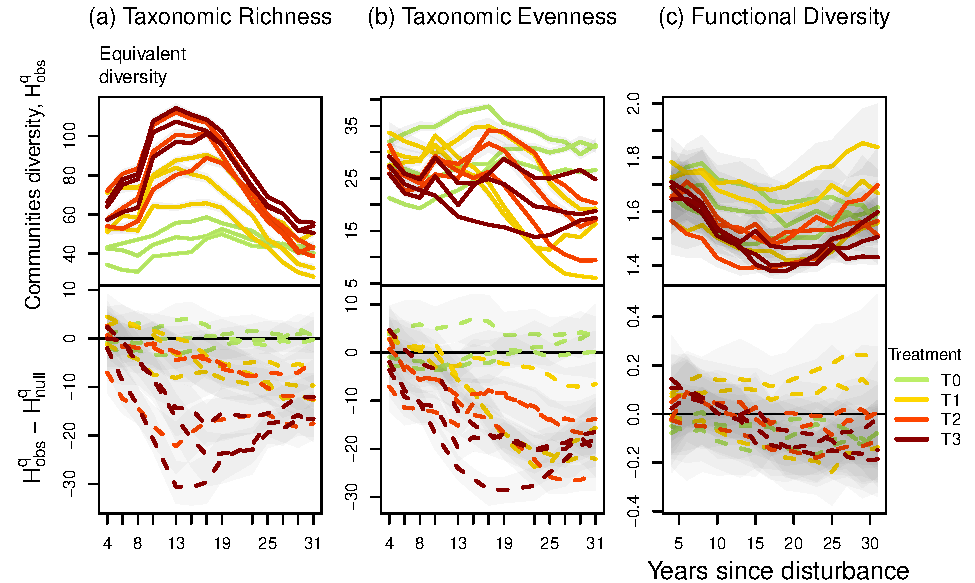
\includegraphics{RecruitmentTrajectories_files/figure-latex/DivTraj-1} 

}

\caption{Upper panels, trajectories over 30 years of taxonomic richness \textbf{(a)}, taxonomic evenness \textbf{(b)} and functional diversity \textbf{(c)} of observed 2-years laps recruitment $H_{obs}^q$. Lower panels, diversity differences to null models $H_{obs}^q - H_{null}^q$. Shaded areas are the credibility intervals.}\label{fig:DivTraj}
\end{figure*}

\subsection{Functional composition}\label{functional-composition}

In undisturbed plots functional traits values remained stable over the
30 years while it followed hump-shaped trajectories in all disturbed
plots, to the exception of the leaf chlorophyll content. Trajectories of
SLA and bark thickness first increased before decreasing towards initial
values. Conversely, trajectories of leaf thickness, leaf toughness, wood
specific gravity, and maximum height first decreased and then started
returning towards initial values but their recovery remained unachieved
after 30 years (Figure \ref{fig:CWM}).

\begin{figure*}

{\centering 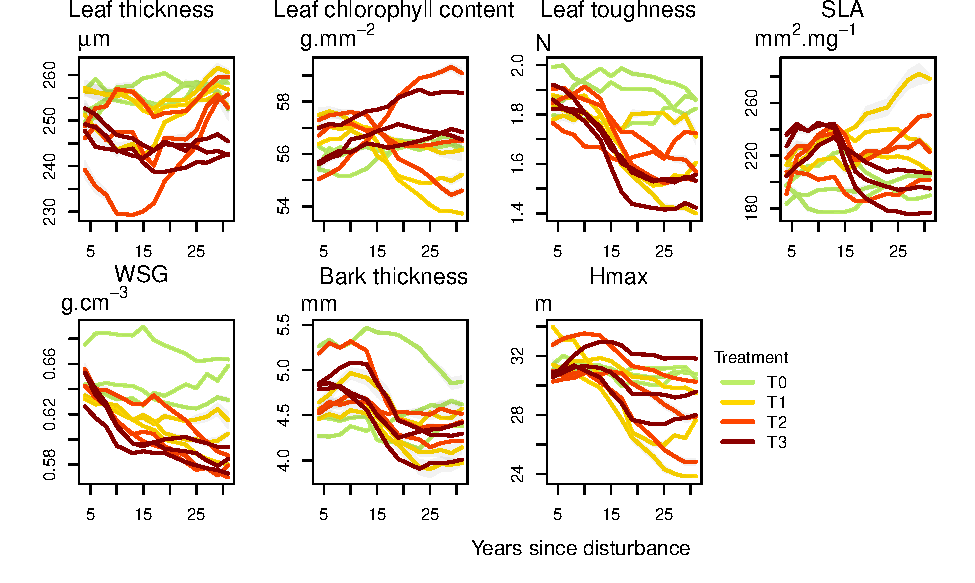
\includegraphics{RecruitmentTrajectories_files/figure-latex/CWM-1} 

}

\caption{Community weighted means (CWM) of the 7 functional traits considered: leaf thickness, leaf chlorophyll content, leaf tougness, specific leaf area (SLA), wood specific gravity (WSG), bark thickness and maximum height at adult stage (Hmax). Shaded areas are the credibility intervals.}\label{fig:CWM}
\end{figure*}

\subsection{Recruitment Turnover}\label{recruitment-turnover}

Over the 30 years in control plots the turnover of recruited species
compared to initial community remained low (Figure \ref{fig:Turnover}).
In disturbed plots the recruited species turnover followed a marked
hump-shaped trajectory, with a maximum reached around 15 years after
disturbance. The maximum turnover was positively correlated to the
disturbance intensity (\(\rho_{spearman}=0.93\)). Thirty years after
disturbance the turnover had returned to low values.

\begin{figure}

{\centering 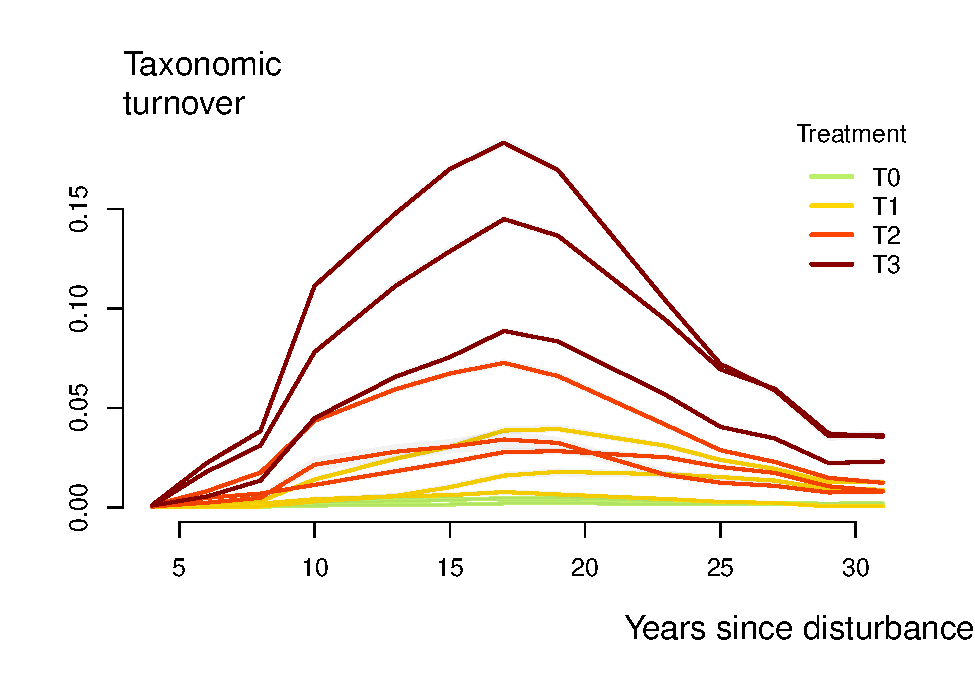
\includegraphics[width=1\linewidth]{RecruitmentTrajectories_files/figure-latex/Turnover-1} 

}

\caption{Trajectories over 30 years of the abundance-based turnover between 2-years laps recruited trees pre-disturbance communities.}\label{fig:Turnover}
\end{figure}

\section{Discussion}\label{discussion}

Our analysis of the taxonomic and functional response of tree
recruitment over 30 years following a disturbance gradient highlighted a
three-phased successional pathway shaped by an interplay between
stochastic recruitment and deterministic processes. Although the
recruitment trajectories suggested community taxonomic and functional
recovery, this remained unachieved after 30 years.

\subsection{A three-phased deterministic successional
pathway}\label{a-three-phased-deterministic-successional-pathway}

Post-disturbance recruitment trajectories followed a three-phased
successional pathway defined by the emergence of deterministic
competition processes for light. Following disturbance these processes
balanced stochastic ones, corresponding to species a random recruitment
of species regardless of their functional characteristics as it was
observed in undisturbed communities.

A first phase (0-8 years), defined by a very low taxonomic turnover
between recruited trees and initial communities, corresponded to the lag
before the disturbance impact translated into changes in the recruited
communities (Figure \ref{fig:Turnover}). Recruitment taxonomic and
functional trajectories matched the trajectories of the null model, so
species functional strategy did not influence their recruitment (Figure
(\ref{fig:DivTraj})). The first phase would correspond to the
recruitment of pre-disturbance surviving saplings (DBH \textless{} 10
cm), grown and almost settled before disturbance and corresponding to
late-successional species. These species display
``resource-conservative'' functional strategies, \emph{i.e.} dense leaf
and wood tissues and low exchange surface, favored in undisturbed
communities where light levels are low \citep{Peet1992, Denslow2000}.
These saplings were the first to benefit from the alleviated competition
and the higher light availability that is known to follow disturbance
and foster plant productivity and growth
\citep{Monteith1972, Chazdon1984}.

A second phase (8-15 years) was marked by an increase of the taxonomic
turnover between recruited trees and initial communities, a decrease of
recruits richness and evenness compared to the null model, and a shift
in recruits functional composition towards more ``resource-acquisitive''
strategies. This would mark the recruitment of trees germinated from
seeds, that will eventually represent the main part of the recruitment
\citep{Lawton1988}. The time elapsed since disturbance corresponded to
the time for these pioneers to reach a 10cm DBH and to dominate the
recruited community, which decreased recruits taxonomic richness and
evenness and made the recruitment trajectories depart from those of the
null model. Recruitment processes then changed after disturbance, with
the emergence of deterministic processes favoring a restricted pool of
species. During this second phase, the functional composition of the
recruited community changed towards more ``resource-acquisitive''
functional strategies (Figure (\ref{fig:CWM})), \emph{i.e.} high SLA and
low maximum height, leaf toughness and wood specific gravity
\citep{Wright2004, Chave2009b, Herault2011}. Favored species hence
displayed efficient light acquisition (high SLA and leaf chlorophyll
content) and inexpensive, short-lived tissues (low leaf thickness and
toughness, small Hmax and low wood specific gravity and bark thickness).
This confirmed the role of light availability in the post-disturbance
successional pathways, as already demonstrated in temperate and tropical
forests \citep{Pena2008, Carreno2012, Kunstler2016, Both2019}. The
balance in recruited communities between pioneers and species from
late-succession, pre-disturbance community determined the difference
between null and observed trajectories. This difference depended on the
disturbance intensity (Figure (\ref{fig:DivTraj})): following low
intensity disturbance (T1 plots), pioneers and late-successional species
were balanced \citep{Bongers2009}. Following intense disturbance (T2 and
T3 plots), deterministic processes prevailed and the composition of
recruited communities rapidly differed from this of the pre-disturbance
community with a high dominance of fast growing pioneers like
\emph{Cecropia spp.} or \emph{Vismia spp.}.

A third recruitment ongoing phase (starting around 15 years) delineated
by a return towards pre-disturbance values of functional diversity and
taxonomic richness but not of taxonomic evenness, while the functional
composition remains altered (Figure (\ref{fig:DivTraj}) \&
(\ref{fig:CWM})). Although recruited species remained mainly
light-demanding, so pioneer species still dominated the recruited
communities, but late-successional ones progressively settled
\citep{Fortunel2014}. This would translate the progressive closing of
forest canopy and the increase competition for light and space
{[}\citet{Peet1992};\citet{Denslow2000};{]} Deterministic recruitment
processes then gradually left room again to stochastic recruitment as
observed in undisturbed forest \citep{Lawton1988, Chave2004}.

\subsection{Community recovery}\label{community-recovery}

Following disturbance, there was a recovery of community taxonomic and
functional composition and of the stochastic recruitment processes
observed for undisturbed communities. This confirmed previous results
from the Paracou experiment, conducted 10 years \citep{Molino2001} and
20 years \citep{Baraloto2012a} after disturbance, where the early signs
of the resilience of pre-disturbance taxonomic and functional
composition recovery had been detected.

Thirty years after disturbance, recruited community taxonomic richness
and evenness returned towards pre-disturbance values and their taxonomic
composition returned towards this of pre-disturbance states. This
maintained community initial diversity and composition and meant a low
recruitment of species absent in the pre-disturbance community,
confirming the importance of dispersal limitation among tropical tree
species \citep{Svenning2005}. Functional composition and diversity
trajectories returned as well towards pre-disturbance values, confirming
the maintenance of community functional diversity and composition
\citep{Fukami2005, Fortunel2014}.

Although community taxonomic and functional recovery was ongoing,
recruits diversity and composition remained altered 30 years after
disturbance. Specifically, the higher the disturbance intensity, the
more presistent the dominance of light-demanding species. This long-term
impact on community composition likely alters community functioning
\citep{Diaz2005}, which raises questions for tropical forests
management. Most valuable species indeed are late-successional species
and their exploitation would require cutting cycles of more than 30
years \citep{Putz2012}.

\section{Conclusion}\label{conclusion}

Post-disturbance recruitment trajectories highlighted a three-phased
deterministic successional pathway driven by the emergence of
trait-based deterministic processes balancing pre-disturbance stochastic
processes and enhancing light-acquisitive species. A first phase would
correspond to the recruitment of pre-disturbance surviving saplings
mirroring the taxonomic and functional diversity and composition of
pre-disturbance communities. A second phase corresponded to the
recruitment of true recruits from germinating seeds belonging to a
restricted pool of pioneers favored by the emergence of competitive
exclusion for light. Above a disturbance intensity threshold, this
second recruitment phase saw the dominance of short-lived, very fast
growing pioneers that drastically changed community composition,
diversity, and likely functioning. A third phase eventually corresponded
to the recovery of of stochastic recruitment processes and to the return
towards pre-disturbance taxonomic and functional characteristics.
Although resilient, recruits diversity and composition remained altered
30 years after disturbance, all the more so that disturbance was
intense. Regarding forest management, our results supported cutting
cycles longer than 30 years and the long-term impacts demonstrated
emphasised the importance of evaluating forest management
sustainability. In this regard, highlighting successional pathways and
the corresponding mechanisms would improve the forecasts of forest
dynamics models.

\section{Acknowledgement}\label{acknowledgement}

We are in debt with all technicians and colleagues who helped setting up
the plots and collecting data over years. Without their precious work,
this study would have not been possible and they may be warmly thanked
here.

\section{Data availability}\label{data-availability}

This article is based upon the dataset of the Paracou station, which is
part of the Guyafor permanent plot network in French Guiana
(Cirad-CNRS-ONF). The dataset is available upon request to the
scientific director (https://paracou.cirad. fr).

\begin{center}\rule{0.5\linewidth}{\linethickness}\end{center}

%----------------------------------------------------------------------------------------
%	REFERENCE LIST
%----------------------------------------------------------------------------------------

\bibliographystyle{mee}
\makeatletter
% The filename has .bib extension the must be eliminated
\filename@parse{references.bib}
% parse stores the file name in base. Extension starts at the first dot, so don't use dots in file names.
\bibliography{\filename@base}
\makeatother


%----------------------------------------------------------------------------------------

\end{document}
